\documentclass[11pt]{article}

\usepackage[a4paper,margin=2.2cm]{geometry}
\usepackage[T1]{fontenc}
\usepackage{lmodern}
\usepackage{booktabs}
\usepackage{graphicx}
\usepackage{microtype}
\usepackage{hyperref}

\setlength{\parindent}{0pt}
\setlength{\parskip}{5pt}
\graphicspath{{../results/}{../results/analysis/}}

\title{Few-Shot Classification with DINOv2 Embeddings\\
\large Evaluation Progress Report}
\author{Computer Vision 2026 Project Team}
\date{October 27, 2026}

\begin{document}
\maketitle

\section{Current State and Evaluation Protocol}

The project classifies the 37 breeds of Oxford-IIIT Pet from $K\in\{1,5,10,20\}$
labeled support images per breed. The committed split reserves the official
test set (3,669 images) for final metrics, uses 740 trainval images for
validation, and samples all support sets from the remaining train pool. Each
configuration uses the same five nested support sets (seeds 0--4), so method
comparisons are paired and there is no train--test overlap.

This report uses the committed per-run CSVs
(\texttt{results/linear\_probe.csv}, \texttt{results/finetune.csv}).
\texttt{src.evaluate} recomputes mean $\pm$ sample standard deviation over the
five seeds, then writes the summary tables and plots. Accuracy and macro-F1
are measured on the test split. Training time covers classifier fitting or
fine-tuning, but not one-time feature extraction.

\section{Completed Experiments}

The following experiments have complete per-run result CSVs and can be
regenerated from the repository:
\begin{itemize}
    \item \textbf{E1}: frozen ImageNet ResNet-50 embeddings with L2-normalized
    multinomial logistic regression. The regularization parameter is chosen on
    the validation split.
    \item \textbf{E5}: ResNet-50 with a new 37-class head and \texttt{layer4}
    fine-tuned using AdamW; BatchNorm layers remain fixed.
    \item \textbf{E6}: full ResNet-50 fine-tuning under the same protocol as E5.
\end{itemize}

Table~\ref{tab:quality} gives the available quality results. The experiment log
also describes DINOv2 experiments E2--E7, but their result CSVs, cached
embeddings, and prediction artifacts are not present in this checkout.
Therefore, they are not included in the quantitative comparison below.

\begin{table}[ht]
\centering
\small
\caption{Test metrics in percent (mean $\pm$ standard deviation over five seeds).}
\label{tab:quality}
\resizebox{\textwidth}{!}{%
\begin{tabular}{llcccc}
\toprule
Method & Metric & $K=1$ & $K=5$ & $K=10$ & $K=20$ \\
\midrule
E1 & Accuracy & 75.8 $\pm$ 2.4 & 87.5 $\pm$ 1.2 & 89.7 $\pm$ 0.7 & \textbf{90.9 $\pm$ 0.5} \\
E1 & Macro-F1 & 74.2 $\pm$ 2.6 & 87.2 $\pm$ 1.4 & 89.4 $\pm$ 0.8 & \textbf{90.7 $\pm$ 0.5} \\
E5 & Accuracy & 48.5 $\pm$ 2.7 & 81.7 $\pm$ 1.3 & 86.3 $\pm$ 1.4 & 89.2 $\pm$ 0.4 \\
E5 & Macro-F1 & 46.9 $\pm$ 3.3 & 81.1 $\pm$ 1.4 & 86.0 $\pm$ 1.5 & 89.0 $\pm$ 0.5 \\
E6 & Accuracy & 33.6 $\pm$ 2.9 & 75.9 $\pm$ 2.1 & 82.8 $\pm$ 1.7 & 86.0 $\pm$ 1.3 \\
E6 & Macro-F1 & 31.6 $\pm$ 2.7 & 75.4 $\pm$ 2.0 & 82.3 $\pm$ 2.0 & 85.7 $\pm$ 1.3 \\
\bottomrule
\end{tabular}
}
\end{table}

\section{Preliminary Comparison}

E1 is the strongest verified approach at every shot count. At $K=1$, it is
27.3 percentage points more accurate than E5 and 42.2 points more accurate
than E6. The gap becomes smaller with more labeled support images, but remains
at $K=20$: E1 exceeds E5 by 1.6 points and E6 by 4.9 points.

The efficiency comparison supports the same practical conclusion. At $K=20$,
E1 trains 75,813 parameters in $1.24\pm0.20$ seconds on CPU. E5 trains
15.04M parameters in $132.50\pm0.68$ seconds on CUDA, and E6 trains all
23.58M parameters in $211.58\pm0.17$ seconds on CUDA. All three use the same
23.58M-parameter ResNet-50 backbone, whose forward pass at $224\times224$
costs 8.17 GFLOPs.

\begin{figure}[ht]
\centering
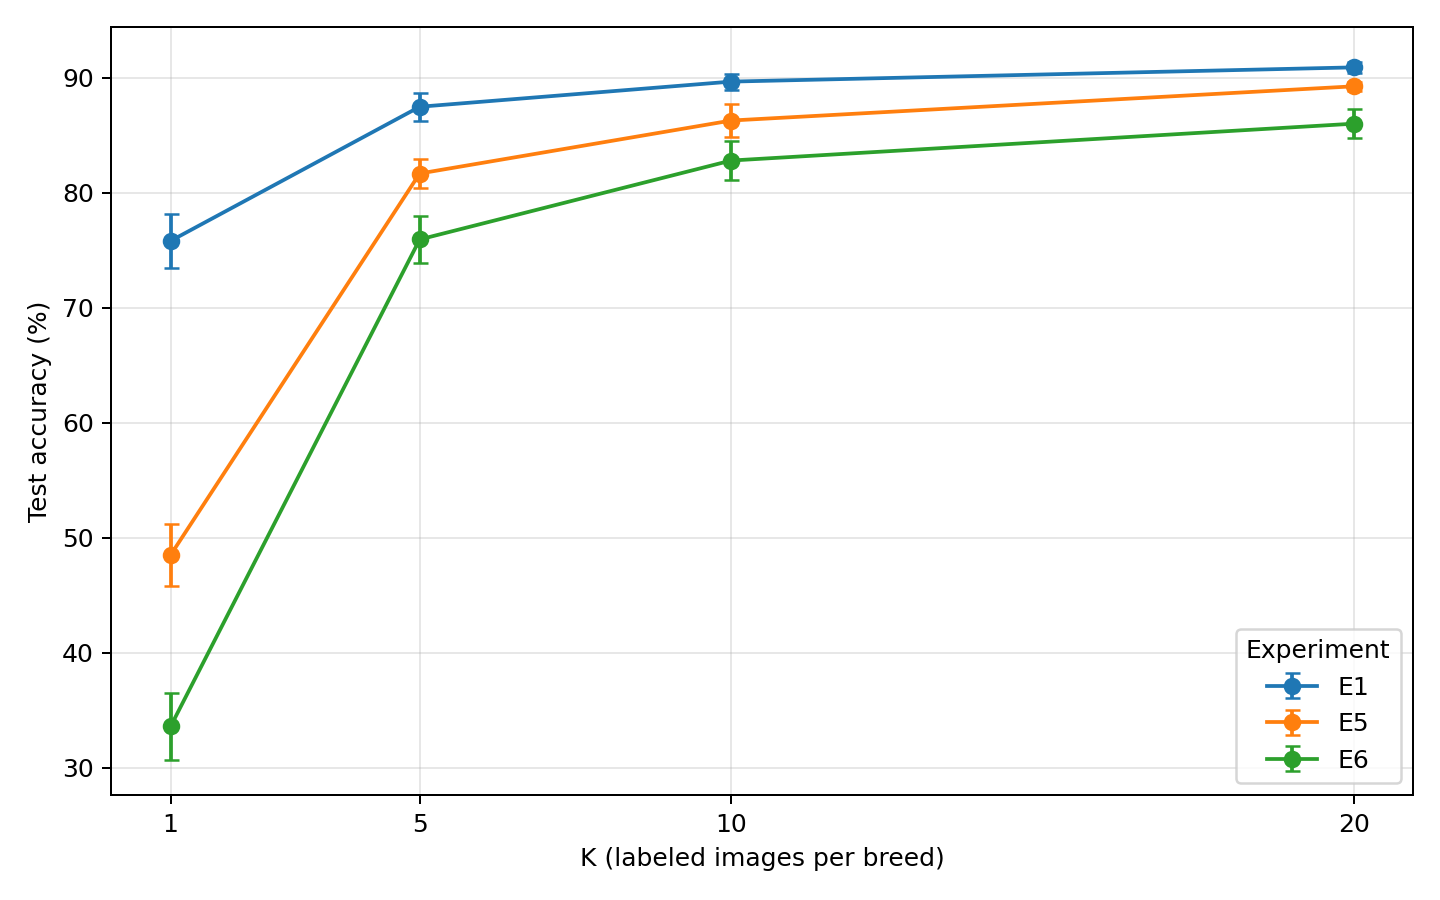
\includegraphics[width=0.49\textwidth]{accuracy_vs_k.png}
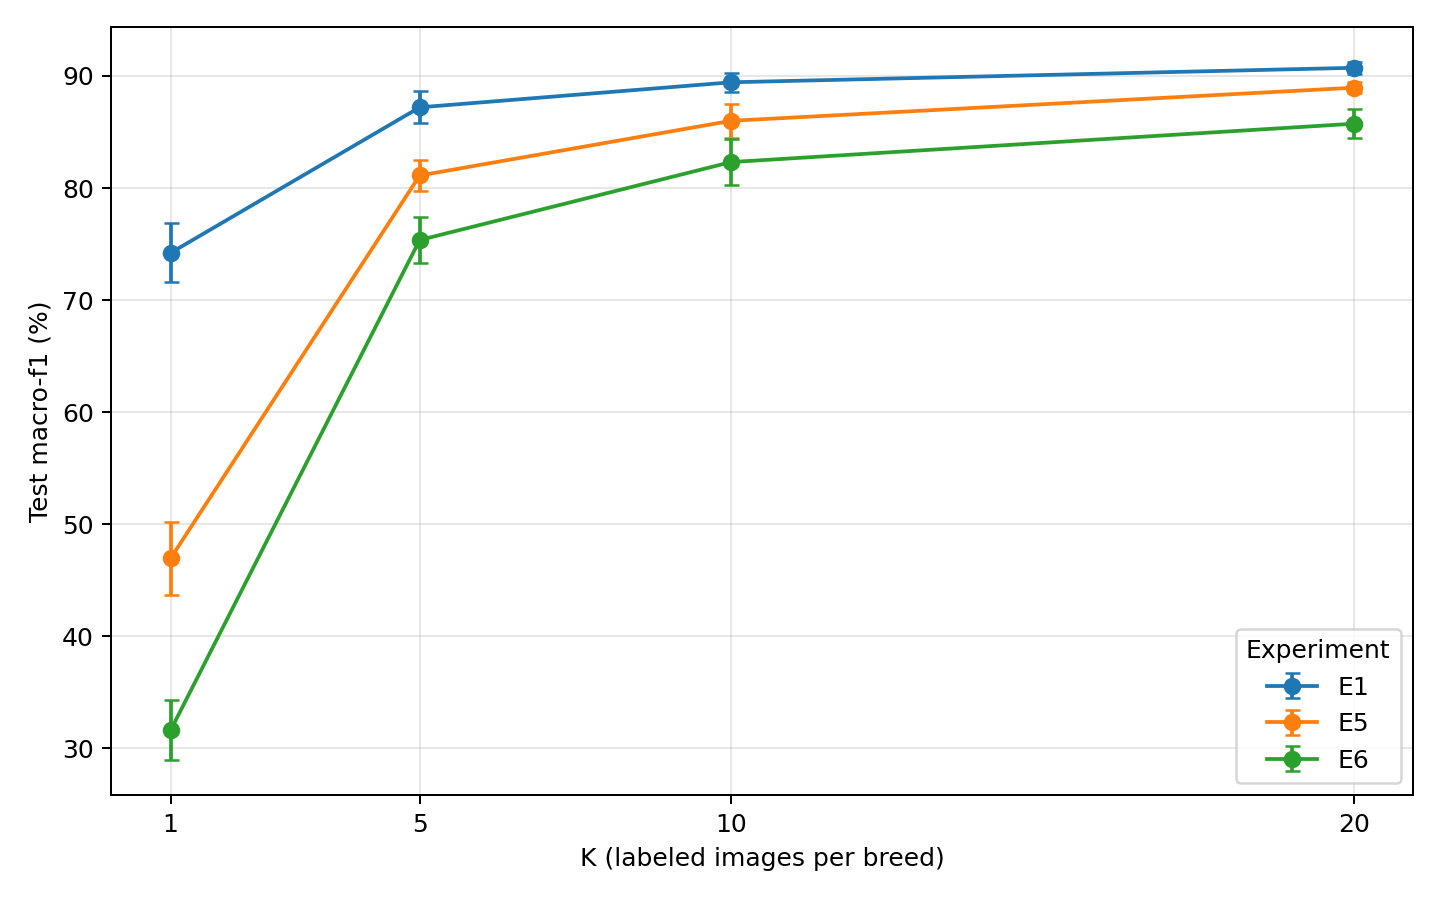
\includegraphics[width=0.49\textwidth]{macro_f1_vs_k.png}
\caption{Available test-set quality metrics. Error bars show the sample
standard deviation across the five support-set seeds.}
\label{fig:curves}
\end{figure}

\section{Observations and Difficulties}

\begin{itemize}
    \item Training fewer parameters is consistently better in the available
    few-shot setting. This is evidence that fine-tuning the ResNet-50 backbone
    overfits, especially when only 37 labeled images are available at $K=1$.
    \item Macro-F1 tracks accuracy closely for every result, so the observed
    ranking is not explained by a few dominant classes in the nearly balanced
    test split.
    \item The validation set has 740 images, which is larger than the $K=1$
    support set. This makes hyperparameter and epoch selection fair across the
    compared methods but may make absolute few-shot performance optimistic.
    \item The validation-best checkpoint is E5 with $K=20$, seed 1: validation
    accuracy is 93.5\%, while its test accuracy and macro-F1 are 89.1\% and
    89.0\%, respectively. This validation--test gap reinforces the need to
    report test metrics rather than validation metrics.
    \item The K=20 E5 seed-4 analysis exposes substantial breed-level errors:
    American Pit Bull Terrier (35\% accuracy), Ragdoll (38\%), British
    Shorthair (69\%), American Bulldog (72\%), and Chihuahua (73\%) are the
    five hardest breeds in that representative run.
    \item The most frequent confusions are American Pit Bull Terrier $\to$
    Staffordshire Bull Terrier (38 images), Ragdoll $\to$ Birman (34), and
    American Bulldog $\to$ Boxer (24). These pairs are visually similar breed
    families; the selected errors have confidence above 99.9\%, indicating
    overconfident mistakes rather than low-confidence ambiguity.
\end{itemize}

\section{Per-Breed Failure Analysis}

The representative $K=20$ E5 run uses seed 4. Figure~\ref{fig:confusion} and
\texttt{results/analysis/} store the per-breed table, confusion matrix, and the
three most frequent misclassification pairs. American Pit Bull Terrier is often
predicted as Staffordshire Bull Terrier; both are compact, short-haired,
muscular terriers and the nearest-support cosine similarity is 0.869. Ragdoll
is confused with Birman (cosine 0.929), which is consistent with their
colourpoint coats and long fur. American Bulldog is confused with Boxer (cosine
0.959), another short-haired, stocky breed. These are plausible visual causes.
The original image paths are not stored in the repository, so the image panels
still need a local dataset copy before stronger claims about pose, occlusion,
clutter, or image quality.

\begin{figure}[ht]
\centering
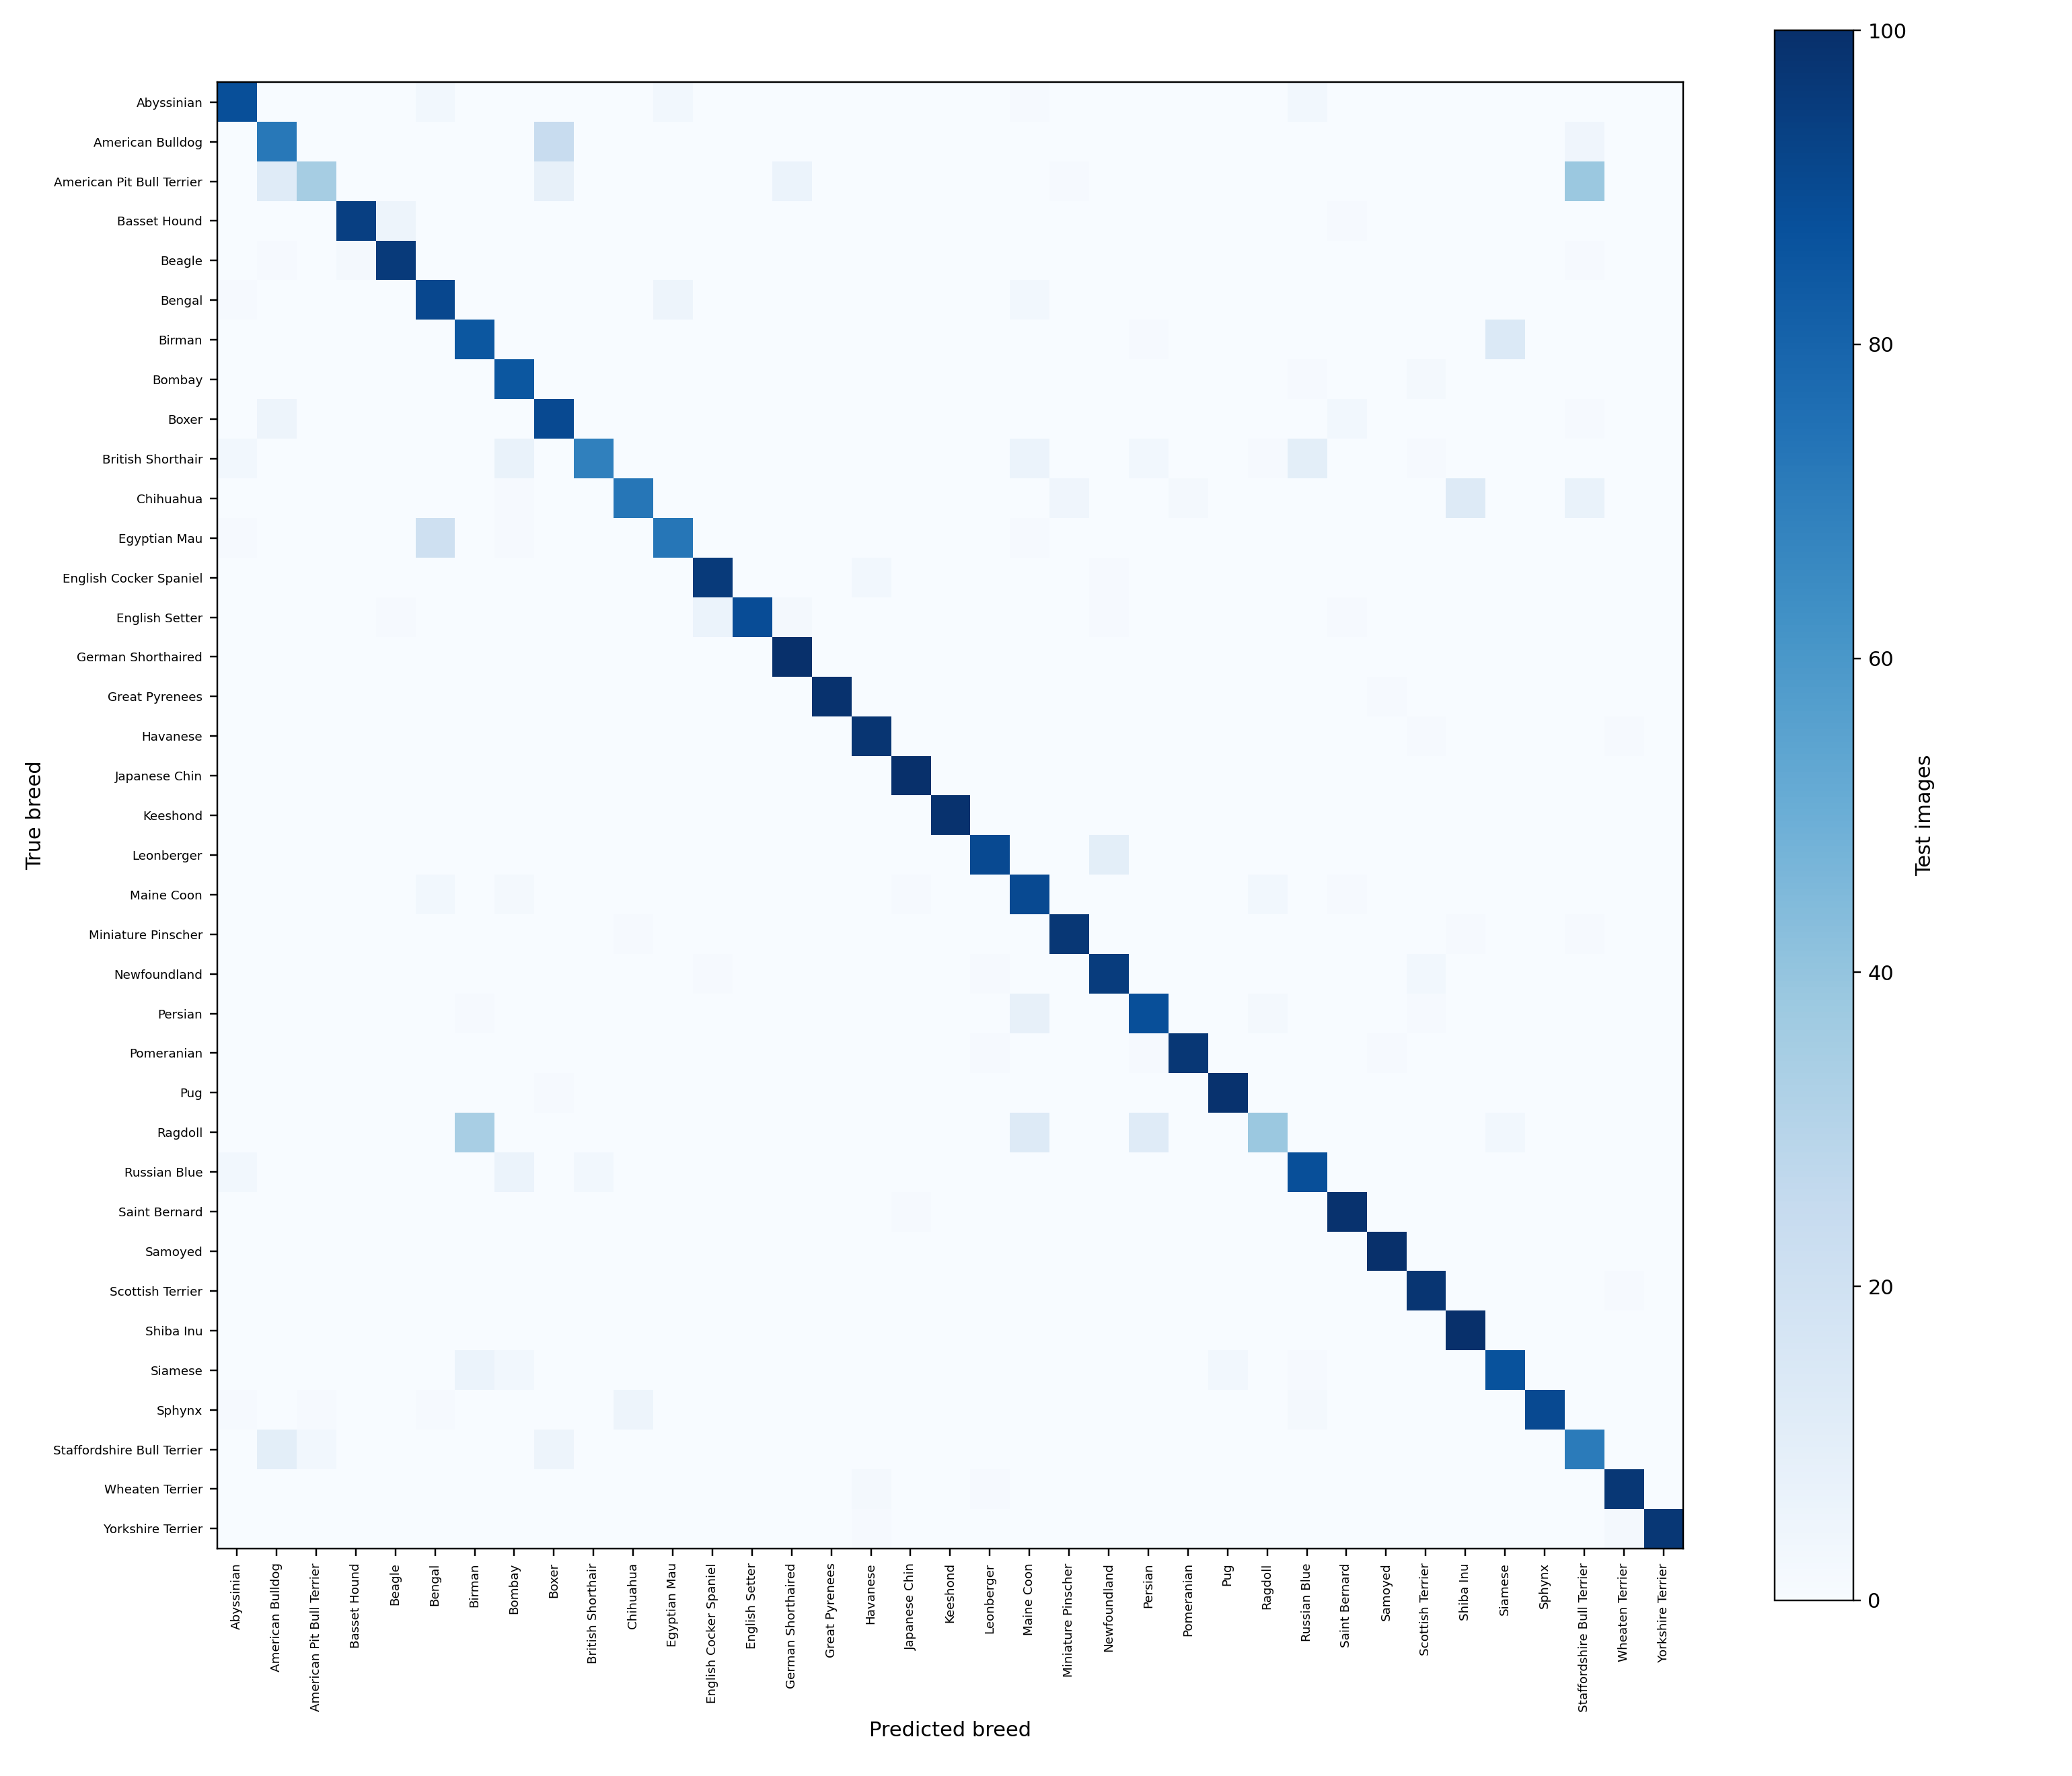
\includegraphics[width=0.92\textwidth]{E5_k20_seed4_confusion.png}
\caption{Confusion matrix for E5, $K=20$, seed 4. The darkest off-diagonal
blocks are the three breed-family confusions listed above.}
\label{fig:confusion}
\end{figure}

\section{Remaining Work}

\begin{enumerate}
    \item Restore or rerun E2--E7 and retain one complete metric CSV per
    experiment, including all $K$ values and five seeds.
    \item Implement the equivalent prediction export for frozen DINOv2
    classifiers so the per-breed and failure analysis compares the main DINOv2
    condition with the ResNet baseline.
    \item Restore the original test and support images for the three saved
    failure cases and annotate concrete visual causes (similar breeds, pose,
    occlusion, multiple animals, clutter, or low resolution).
    \item Complete the final DINOv2-versus-ResNet comparison only after these
    reproducible artifacts are available.
\end{enumerate}

\section{Reproducibility}

Set up the project with \texttt{uv sync}. After the per-run CSVs exist, run
\texttt{uv run python -m src.evaluate}. The evaluator reads those CSVs,
rejects groups without exactly five seeds, and writes
\texttt{summary\_metrics.csv}, \texttt{efficiency\_k20.csv}, and the two curves
in Figure~\ref{fig:curves}. It does not retrain models. Optional checkpoint
analysis (\texttt{--checkpoint E5 20 4}) needs saved weights and the dataset.

\end{document}
